\section{Reconsidering governance and security management}
\subsection{Threat modeling and security requirements}
\setcounter{figure}{2}
In parallel to the investigation by JFSA, we conducted making a document on security management of cryptocurrency exchange right after the CoinCheck incident.
% One of the author of this paper is a member of this group.
%The purpose of the study is collecting practices of constructing and operating the cryptocurrency exchange.
%
Even now, there is no standardized architecture and implementation of software/hardware for cryptocurrency exchange. Therefore, we cannot edit one standard document toward secure implementation and operation of cryptocurrency exchange. The group gathered information of real cryptocurrency exchanges from their engineers, then create a model of cryptocurrency exchange system. Fig.~\ref{fig_system_model}. shows an example of system model of cryptocurrency exchange.
% \begin{figure}
%  \begin{center}
%   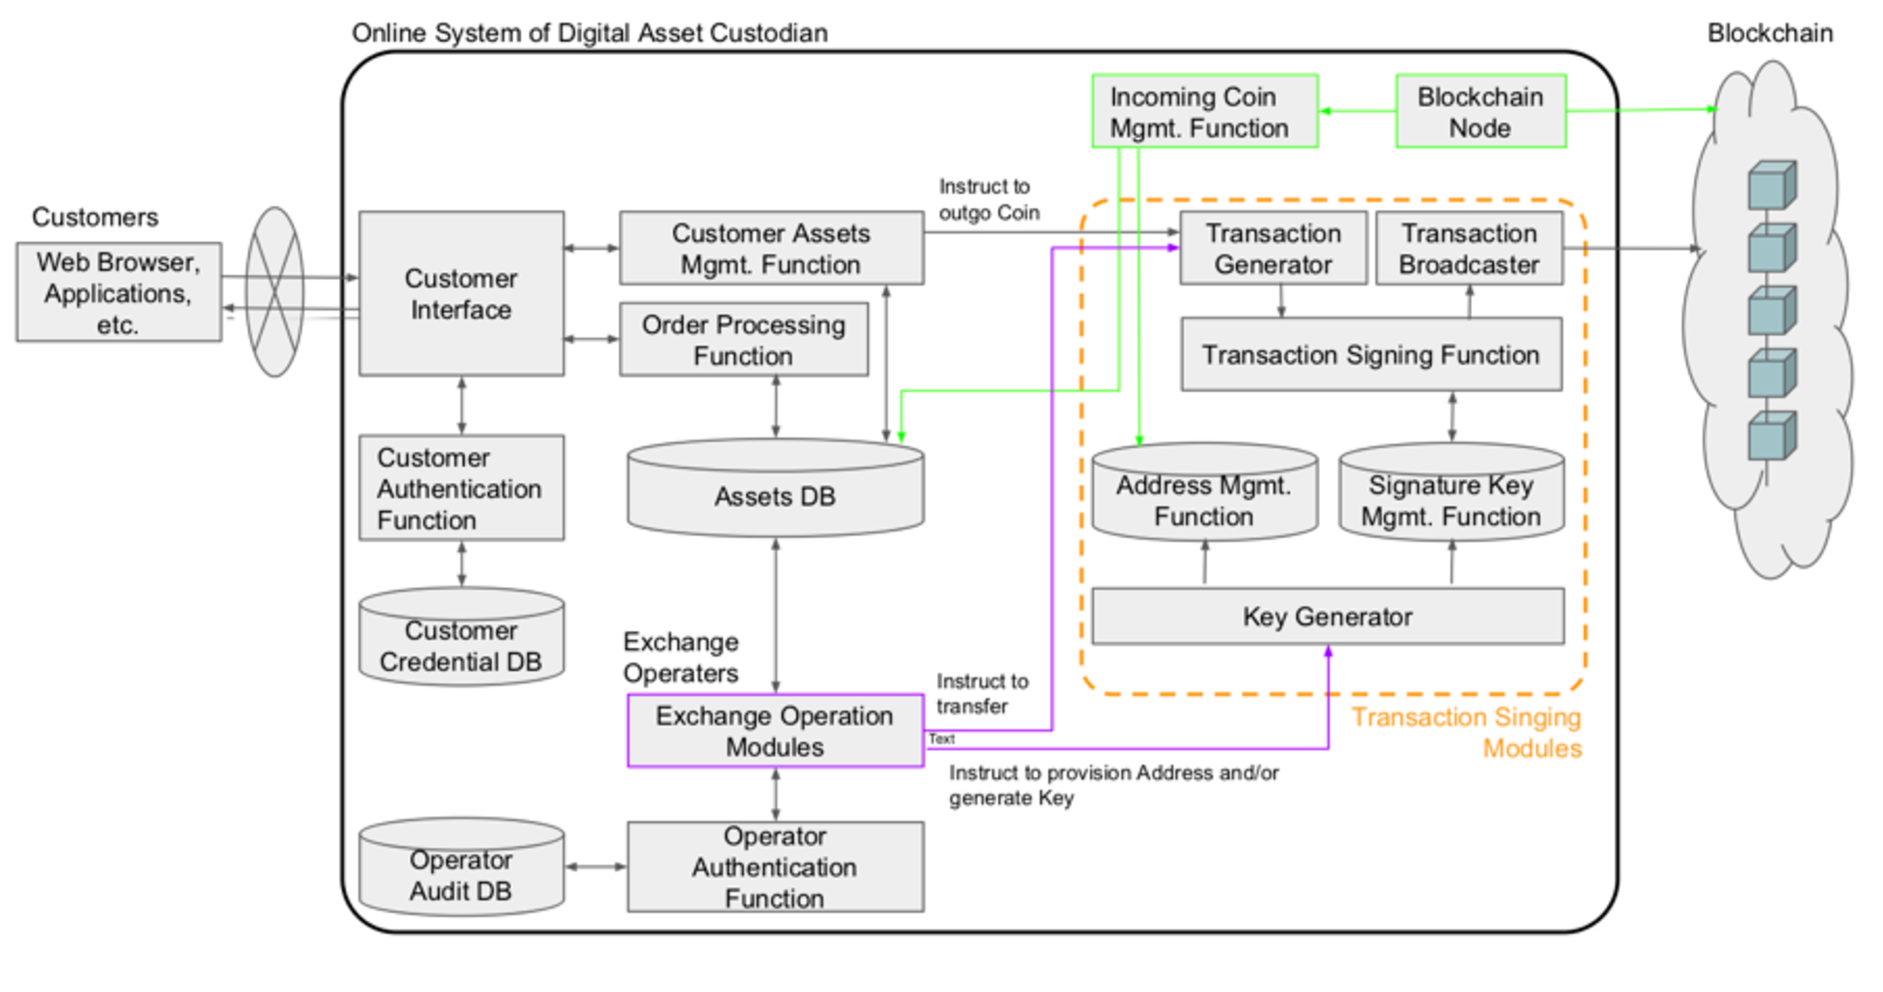
\includegraphics[width=8cm,pagebox=cropbox,clip]{system_model.pdf}
%   \caption{System model of cryptocurrency exchange}
%   \label{fig_system_model}
%  \end{center}
% \end{figure}
%
% \begin{figure}
%  \begin{center}
%   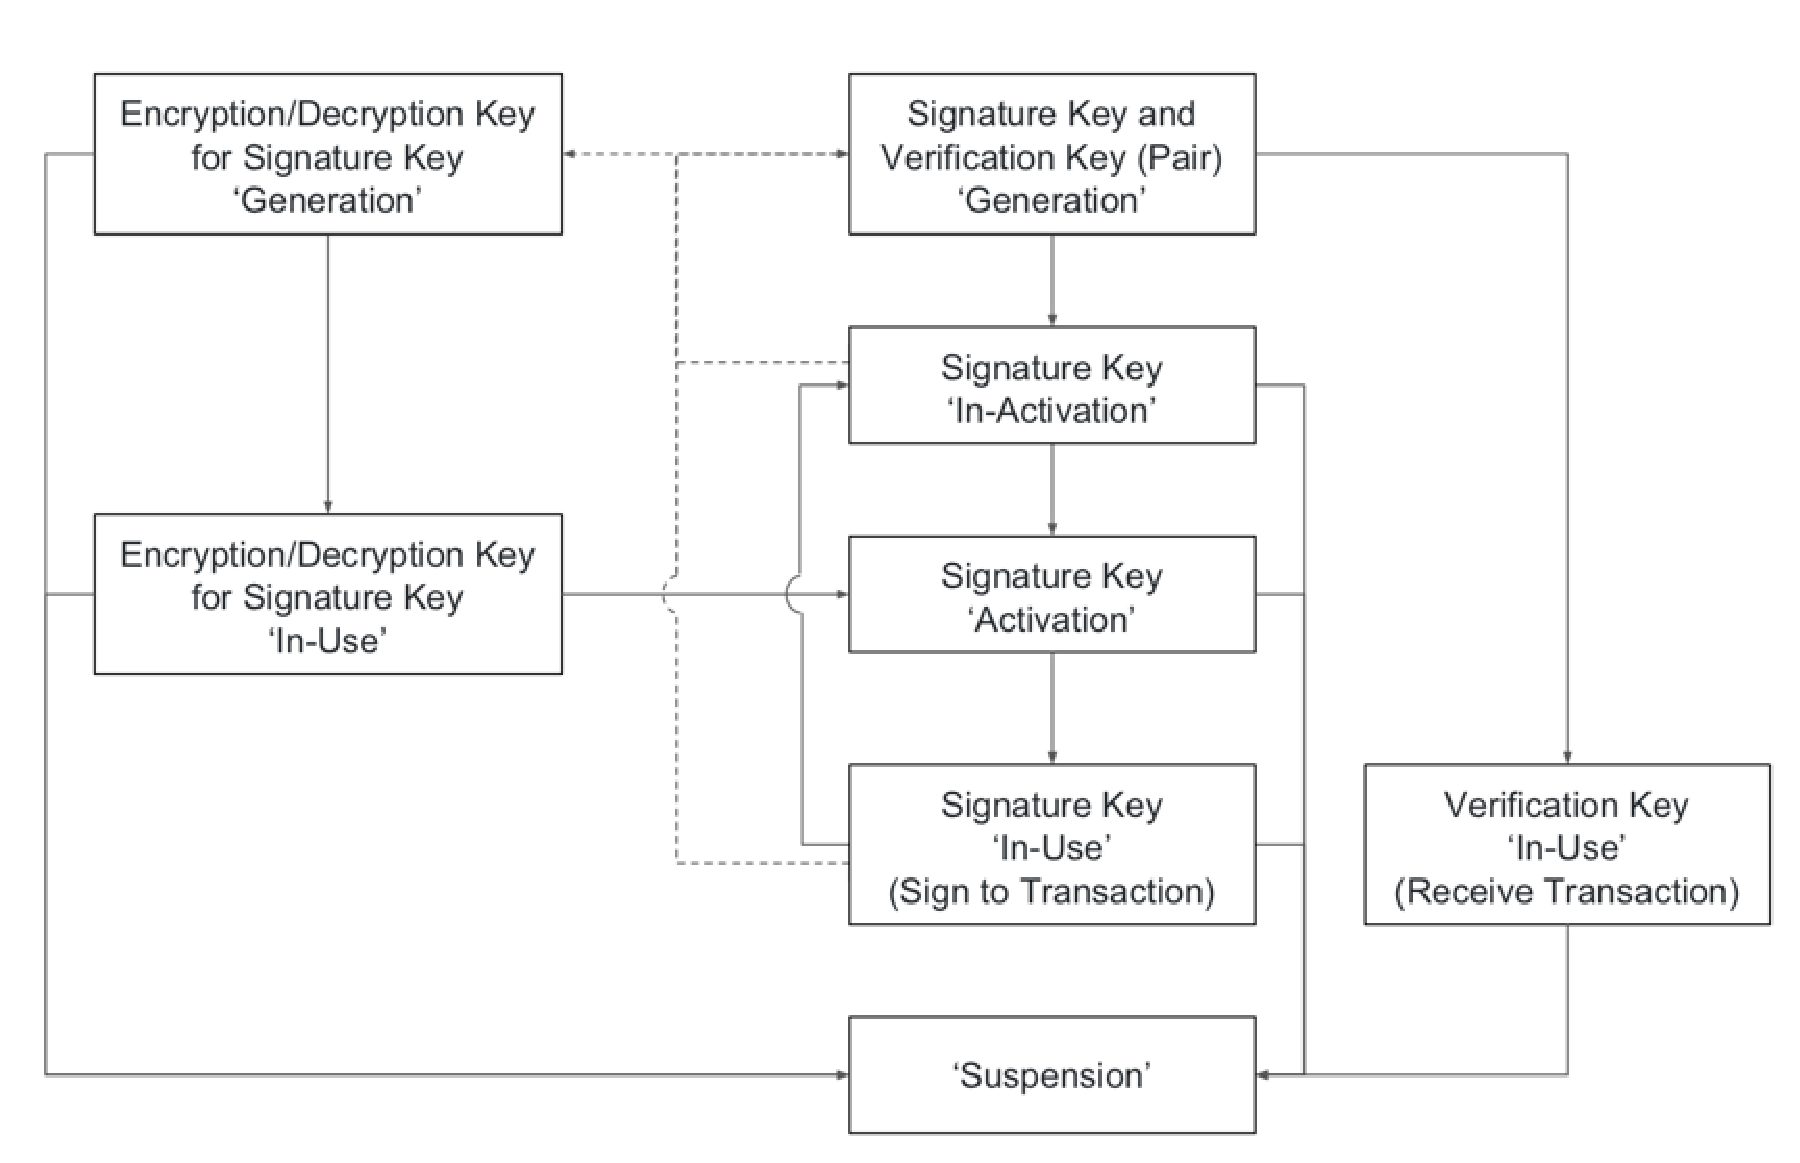
\includegraphics[width=8cm,pagebox=cropbox,clip]{key_lifecycle.pdf}
%   \caption{Key life-cycle at cryptocurrency exchange}
%   \label{key_lifecycle}
%  \end{center}
% \end{figure}
\begin{figure}[htbp]
  \begin{tabular}{cc}
    \begin{minipage}{0.5\hsize}
      \begin{center}
        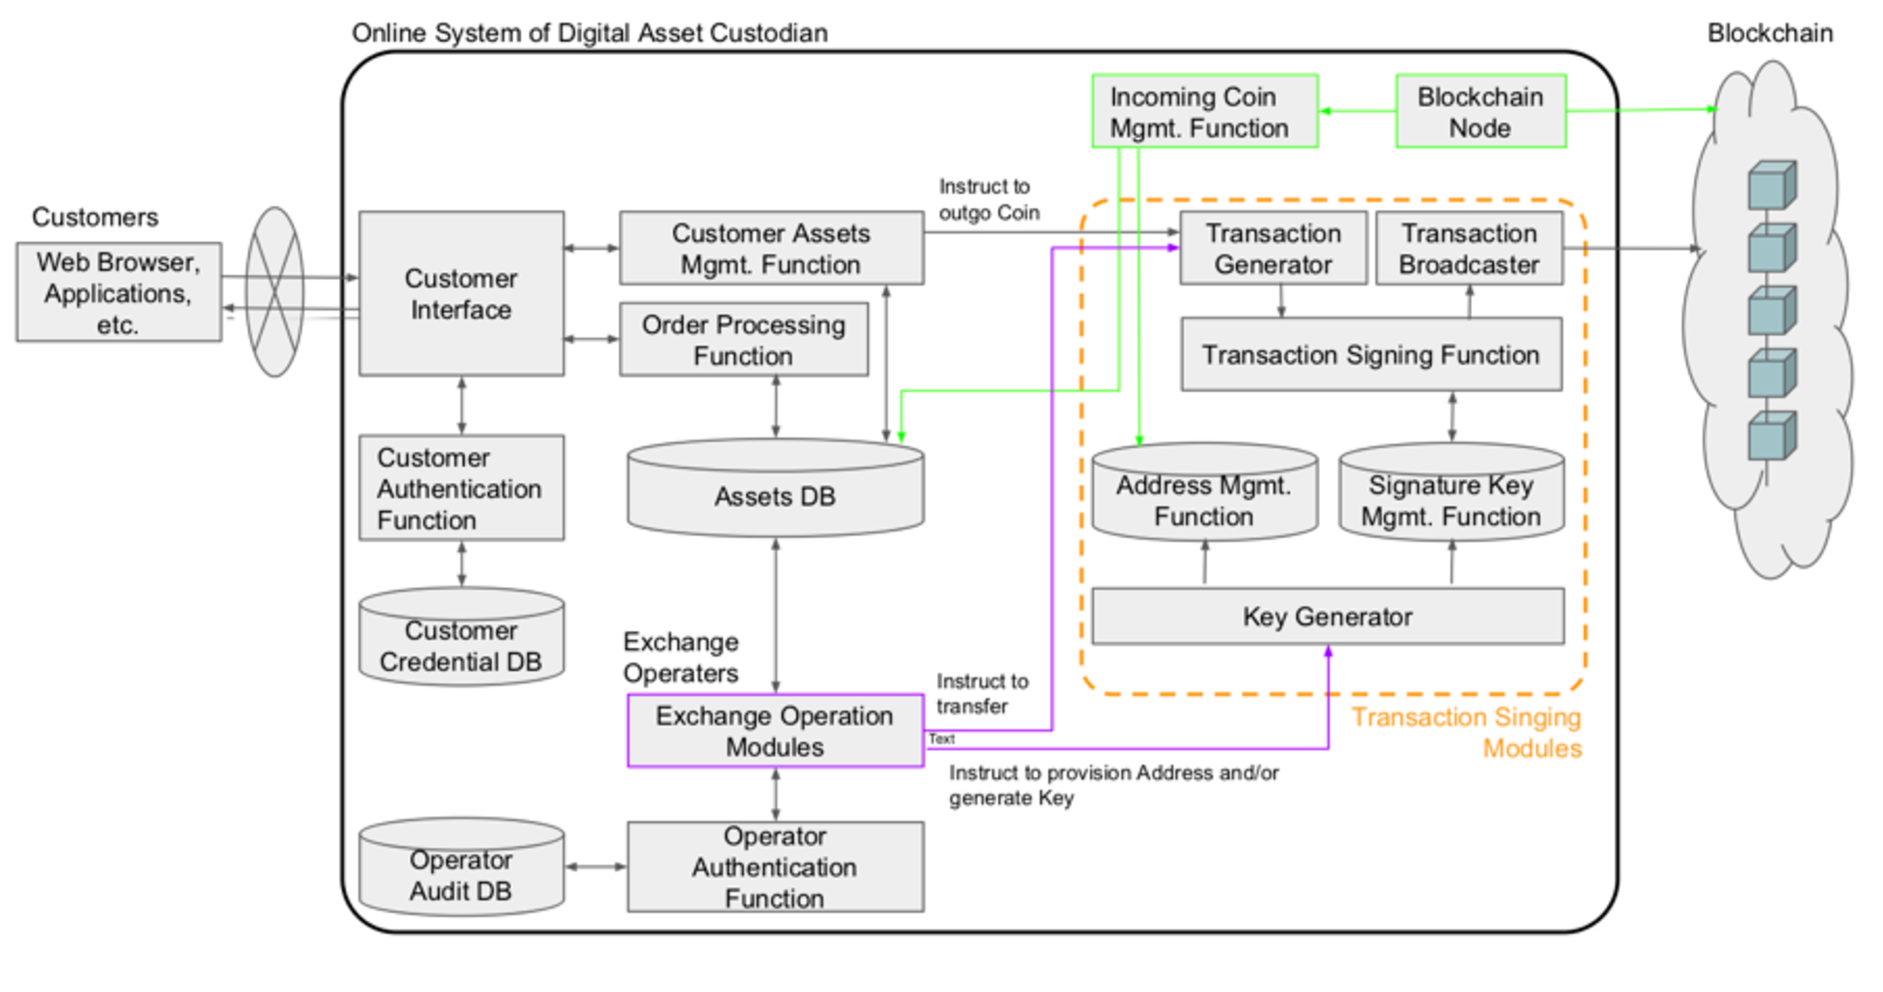
\includegraphics[width=6.5cm,pagebox=cropbox,clip]{system_model.pdf}
        \caption{System model of cryptocurrency exchange}
        \label{fig_system_model}
      \end{center}
    \end{minipage}
    \begin{minipage}{0.5\hsize}
      \begin{center}
        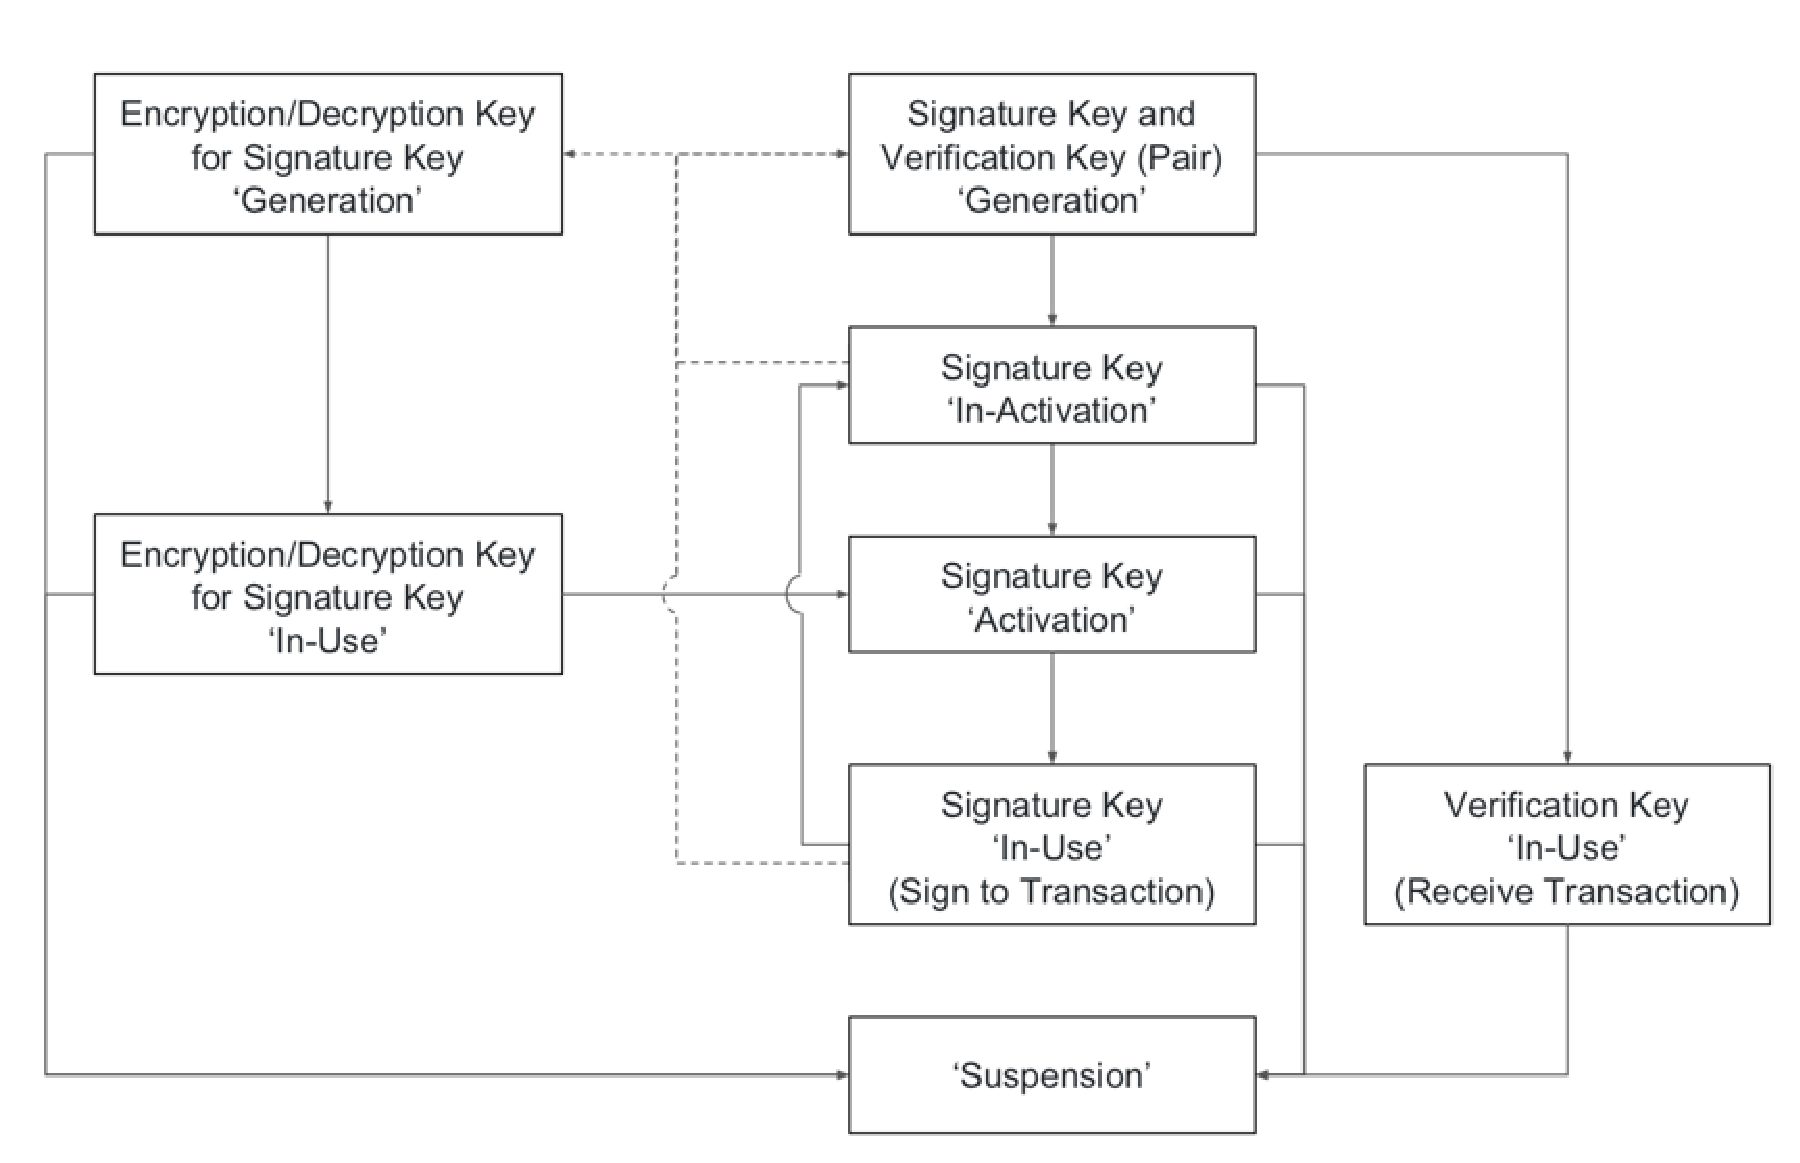
\includegraphics[width=4.5cm,pagebox=cropbox,clip]{key_lifecycle.pdf}
        \caption{Key life-cycle at cryptocurrency exchange}
        \label{key_lifecycle}
      \end{center}
    \end{minipage}
  \end{tabular}
\end{figure}


The model consists of Customer Interface for UI for login and transaction, Customer Authentication Function, Customer Credential Database, Customer Assets Management Function, Blockchain Node for incoming transactions, Incoming transaction management Function, Order processing function, Assets Database, Transaction Singing Function for outgoing transactions, Exchange Operation Modules, Operator Authentication Function and Operator Audit Database.
%Details are described in Appendix~\ref{appendix_system_model}
We defined each functional element to distinguish functions logically, and do not show the actual arrangement on the actual system.
%For example, in our actual system, address management unit may be managed by an integrated database. Also, there are implementations with multiple functions packaged together. For example, each functional element of the transaction signature system may be integrated with the customer property management system, or the transaction signature system may be operating as another system.
\begin{table}
 \caption{Keys in cryptocurrency exchange}
 \begin{tabular}{ll} \hline
  Types                     & Description                                             \\ \hline
  Signature Key             & A private key for signing transactions                  \\
                            & (asymmetric key cryptography)                           \\ \hline
  Verification Key          & A public key for verification of transactions           \\ % (asymmetric  \\
                            & (asymmetric key cryptography)                           \\ \hline% Recipient address of transactions
  % &  are unique value calculated from verification key) \\ \hline
  Encryption/decryption key & Secret key to keep confidentiality of signature key     \\
  for signature key         & (symmetric key cryptography)                            \\ \hline

  Master Seed               & A seed to generate a signature key in decisional wallet \\ \hline
 \end{tabular}
 \label{tbl_4_1}
\end{table}
After a pair of a signature key and a verification key (hereafter “key pair”) is generated, an address to receive transactions is generated from the verification key. By notifying a sender of crypto assets this address, the sender is able to transfer the asset to the address. When the recipient transfers the asset to the other address, the original recipient signs the transaction data which includes the transfer order. Inactive state of the signature key is the state such that the signature key is stored in confidential manner in the signature key management function of Fig.~\ref{fig_system_model}. An example of inactivation is encryption by encryption/decryption key (e.g. pass phrase), that is, the signature key is encrypted. In contrary, activation is the process to make the key usable to sign, by decrypting the inactivated key. The activation is assumed to be executed in transaction signing function of Fig.~\ref{fig_system_model}. Activation and inactivation may be executed in an implementation of wallet, when the wallet have both functions. The signature key is not needed after its generation until execution of signing to transaction. Thus, there is a way to manage the signature key in offline manner with storing the verification key and address online(cold wallet).

\begin{description}
 \item[On the usage of multiple keys:]
       In some crypto assets system, it is recommended not to use the same key pair twice, thus it produces multiple key pairs. This feature is for preventing trace and not relevant to the business efficiency of a cryptocurrency exchange.
       %However, a cryptocurrency exchange should manage addresses for each customer. Thus it should manage multiple key pairs for the same crypto assets.
 \item[On the suspension of keys:]
       Suspension of key usage is only an operation inside a cryptocurrency exchange. By definition of blockchain based crypto assets system, any user cannot cancel transaction once it is made. As another case, it is difficult to revoke signature key even after the suspension of key. For example, a customer accidentally operate some crypto assets for suspended address. In such case, the suspended signature key is needed to make an reimbursement. Thus, suspension of keys should be conducted with considering such cases.
\end{description}

%In the cryptocurrency exchange, the role and risk of the signing key are extremely large. This is not only to enable the transfer of coins but also to disappear due to the anonymity of the Crypto Asset, the property that it is impossible to revocation the signing key against leakage / theft or roll back the transaction by.
%In this section, we show the risk of fraudulent use that could lead to the loss of the signing key, leakage / theft, and damage of value. It also shows supply chain risk etc. when introducing Wallet related to signature key.

\subsection{Analysis based on security management standard}
%\subsection{Analysis based on governance and security management standard}

%At cryptocurrency exchanges, it is mandatory to establish, conduct, maintain and continuously improve security management. As requirements in term os security management, items described in [ISO.27001:2013] are sufficiently considered according to the business process of each cryptocurrency exchange. Especially, following items should be carefully considered, because a cryptocurrency exchange retains customer’s asset and should deal with issues specific to crypto assets.
\begin{description}
 \item[On stakeholders]\footnote{ISO 27001~\cite{ISO27001} Clause 4}
       It is needed to consider protection of customer’s assets, as well as division of responsibility with outsourcers including security of private key management for crypto asset, and mattes by which a cryptocurrency exchange may give social impacts like money laundering.
 \item[On security policy]\footnote{ISO 27001~\cite{ISO27001} Clause 5}
       A cryptocurrency exchange should define a security policy which includes security objectives and controls. Especially, it is recommended to disclose the security policy on the management of crypto assets to customers to facilitate self evaluation.
 \item[Continuous risk evaluation and improvement]\footnote{ISO 27002~\cite{ISO27002} Clause 6, 8, 9 and 10}
       A cryptocurrency exchange should watch security risks of crypto assets in addition to aligning the general security management framework, because the risks change and increase due to rapid development of related technology. It is especially important to continuously evaluate risk and improve security objectives, policy and controls to keep effectiveness of security controls after starting their operations. A cryptocurrency exchange should decide security objectives and controls with considering viewpoint as countermeasure to threat as lost, theft, leak and abuse of customer’s assets data and private key for crypto assets, requirements for actual business, compliance to laws and rules and social responsibilities to prevent crimes in use of crypto assets like scam and money laundering.
\end{description}
The cryptocurrency exchange conducts threat analysis, vulnerability evaluation, risk evaluation and defining security objectives and controls according to its actual business and system. Security objectives and controls should be decided with considering threats and risks specific to crypto assets, as well as general security objectives and controls described in ISO 27002~\cite{ISO27002}.
%Followings are items of security objectives and controls described in [ISO.27002:2013].
%\begin{itemize}
%  \item Information Security Policies
%  \item Organization of information security
%  \item Human resource security
%  \item Access control
%  \item Cryptography
%  \item Physical and environmental security
%  \item Operations security
%  \item Communications security
%  \item System acquisition, development and maintenance
%  \item Supplier relationships
%  \item Information security incident management
%  \item Information security aspects of business continuity management
%end{itemize}
%Consideration of above items is mandatory. Next close describes specific items to be considered by a cryptocurrency exchange.

\subsubsection{Risk analysis of signing secret key}
Risk analysis differs depending on the assumed threats, system
configuration, threat modeling, and so on.
%In this section, we show
%a case study based on the following assumption as an example.
Here,
the threat concerning the signature secret key and the factors that
can cause the threat are assumed as follows.
%In addition, we assumed
the following as the actor giving input to the signing secret key
based on Fig.~\ref{fig_system_model}% in \ref{Threat modeling and security requirements}.

\begin{itemize}
 \item Threats: lost, leakage, theft and fraudulent use.
       %  \begin{itemize}
       %    \item lost
       %    \item leakage, theft
       %    \item fraudulent use
       %  \end{itemize}
 \item Factors of Threats: mis-operations, legitimate users' malice, spoofing, intrusions from outside and unintended behaviors of implementations.
       %    \begin{itemize}
       %    \item mis-operations
       %    \item Legitimate users' malice
       %    \item Spoofing
       %    \item Intrusions from outside
       %    \item Unintended behaviors of implementations
       %    \end{itemize}
 \item Actors: exchange operation modules, transaction signing modules, customer asset management function implementation and incoming coin management function implementation.
       %  \begin{itemize}
       %     \item exchange operation modules
       %     \item Transaction Signing modules
       %     \item customer asset management function implementation
       %     \item incoming coin management function implementation
       %  \end{itemize}
\end{itemize}

% move to appendix
%  Factors of threats are organized as follows.
%
%  Mis-operation: An act that an authorized user (including an
%  administrator) of the system accidentally operated by mistake.  For
%  example, it is incorrectly supposed that an operation to coin 100,000
%  yen is incorrectly dispatched for 1 million yen.

%  Legitimate users' malice: Acts performed by a legitimate user of the
%  example, theft or unauthorized use of the signature private key due
%  to internal fraud.  In this case, it is the purpose of identifying
%  acts that can be factors, and the purpose and incentive of the act
%  are not limited here.

%  Spoofing: An act other than an authorized user of the system
%  impersonating a legitimate user (more accurately impersonating some
%  kind of operation).  For example, an internal burglar without
%  administrator privilege accesses the system with administrator
%  authority.

%  Intrusions from outside: an act of an outsider accessing the system
%  malicious intrusion from the outside by exploiting the system's
%  vulnerability, incorporating malware into the exchanging system via
%  targeted e-mail to the exchanges' administrator or the like and
%  generating a private signature private key (or transaction creation)
%  from the outside, Allow remote control of etc.

%  Unintended behaviors of implementations: The system behaves
%  unexpectedly by the designer or operator irrespective of the
%  intention or malice of the operation.  For example, a signature
%  private key leaks due to a bug in the exchange management system.
Of these threat factors, theft and fraudulent use are regarded as
threats that can only be caused by explicit malicious factors.
% As a
% result, the possible risks for signing key to be assumed are the
% figured in appendix \ref{appendix_risks}


%Objectives of security management at a cryptocurrency exchange contain secure protection of customer’s asset, compliance to business requirements, laws and rules, and realization of social responsibility. Security policies and execution statements derived from such objectives are recommended to be publicly available for consumers, business partners, auditor and regulators to help their judge.
